% ============================================
% VI. THEORETICAL MAXIMUM THROUGHPUT ANALYSIS
% ============================================
\section{Theoretical Maximum Throughput Analysis}
\label{sec:theoretical}

We formalize a throughput model accounting for both server-side processing and on-chain settlement constraints. The maximum throughput is determined by the minimum of these capacities~\cite{harcholbalter2013performance}:

\begin{equation}
\lambda_{max} = \min(\lambda_{server}, \lambda_{blockchain})
\label{eq:lambda_max}
\end{equation}

\textbf{Blockchain-Side Limit.} The blockchain throughput is constrained by block gas limit ($G_{block}$), gas cost per transaction ($G_{tx}$), and block time ($T_{block}$). With our configuration (10,485,760 gas limit, 4-second blocks, 146,194 gas/tx):

\noindent
\begin{minipage}{0.48\textwidth}
\begin{equation}
\lambda_{blockchain} = \frac{G_{block}}{G_{tx} \cdot T_{block}}
\end{equation}
\end{minipage}%
\hfill
\begin{minipage}{0.48\textwidth}
\begin{equation}
\lambda_{blockchain} = \frac{10{,}485{,}760}{146{,}194 \times 4} \approx 17.93 \text{ tx/sec}
\end{equation}
\end{minipage}

This represents the \textit{sustained} throughput ceiling—the maximum rate at which transactions can be confirmed indefinitely in steady state. However, our observed throughput in Architecture~5 was 31.19~tx/sec with 125 transactions per block, significantly exceeding this limit. This demonstrates the architecture's \textbf{burst handling capability}.

The distinction between \textit{sustained} and \textit{burst} throughput is critical. Trading workloads are inherently bursty: market events generate sudden spikes far exceeding average rates. When transactions arrive faster than the blockchain's sustained capacity, they accumulate in the mempool and confirm across subsequent blocks. Our measured 31.19~tx/sec reflects transactions \textit{submitted and eventually confirmed} over the test duration—1.74$\times$ the sustained capacity (31.19/17.93). In sustained load exceeding 17.93~tx/sec, throughput would converge toward this ceiling as the mempool reaches equilibrium. The key insight: our architecture shifted the bottleneck away from server-side contention, processing transactions faster than the blockchain could confirm them.

\textbf{Server-Side Limit.} Server throughput depends on parallelism and synchronization costs, following Amdahl's Law~\cite{gustafson1988reevaluating} and Little's Law~\cite{little1961proof}:

\begin{equation}
\lambda_{server} = \frac{N}{T_{process} + T_{contention}}
\end{equation}

where $N$ is parallel workers, $T_{process}$ is per-transaction processing time, and $T_{contention}$ is time waiting for shared resources. Architecture~3 (Multi-Threaded, Single-Wallet) had threads contending for the single wallet's nonce, serializing submissions. Architecture~4 (Unsynchronized Multi-Wallet) removed nonce contention but exposed significant server-side contention, with $T_{contention}$ causing 27.2~s average latency.

\textbf{Achieving Theoretical Maximum.} Our components maximize $\lambda_{server}$ so the system becomes purely blockchain-limited. The \textbf{Asynchronous Multi-Wallet Strategy} creates $N$ independent submission lanes, fully utilizing block gas in parallel. The \textbf{Symbol-Sharded Lock-Free Model} partitions processing by symbol, eliminating inter-thread contention ($T_{contention} \to 0$):

\begin{equation}
\lambda_{server} \approx \sum_{i=1}^{N_{shards}} \frac{1}{T_{process, i}}
\end{equation}

Figure~\ref{fig:solution-architecture} shows the complete integrated architecture combining these components.

\begin{figure}[!ht]
\centering
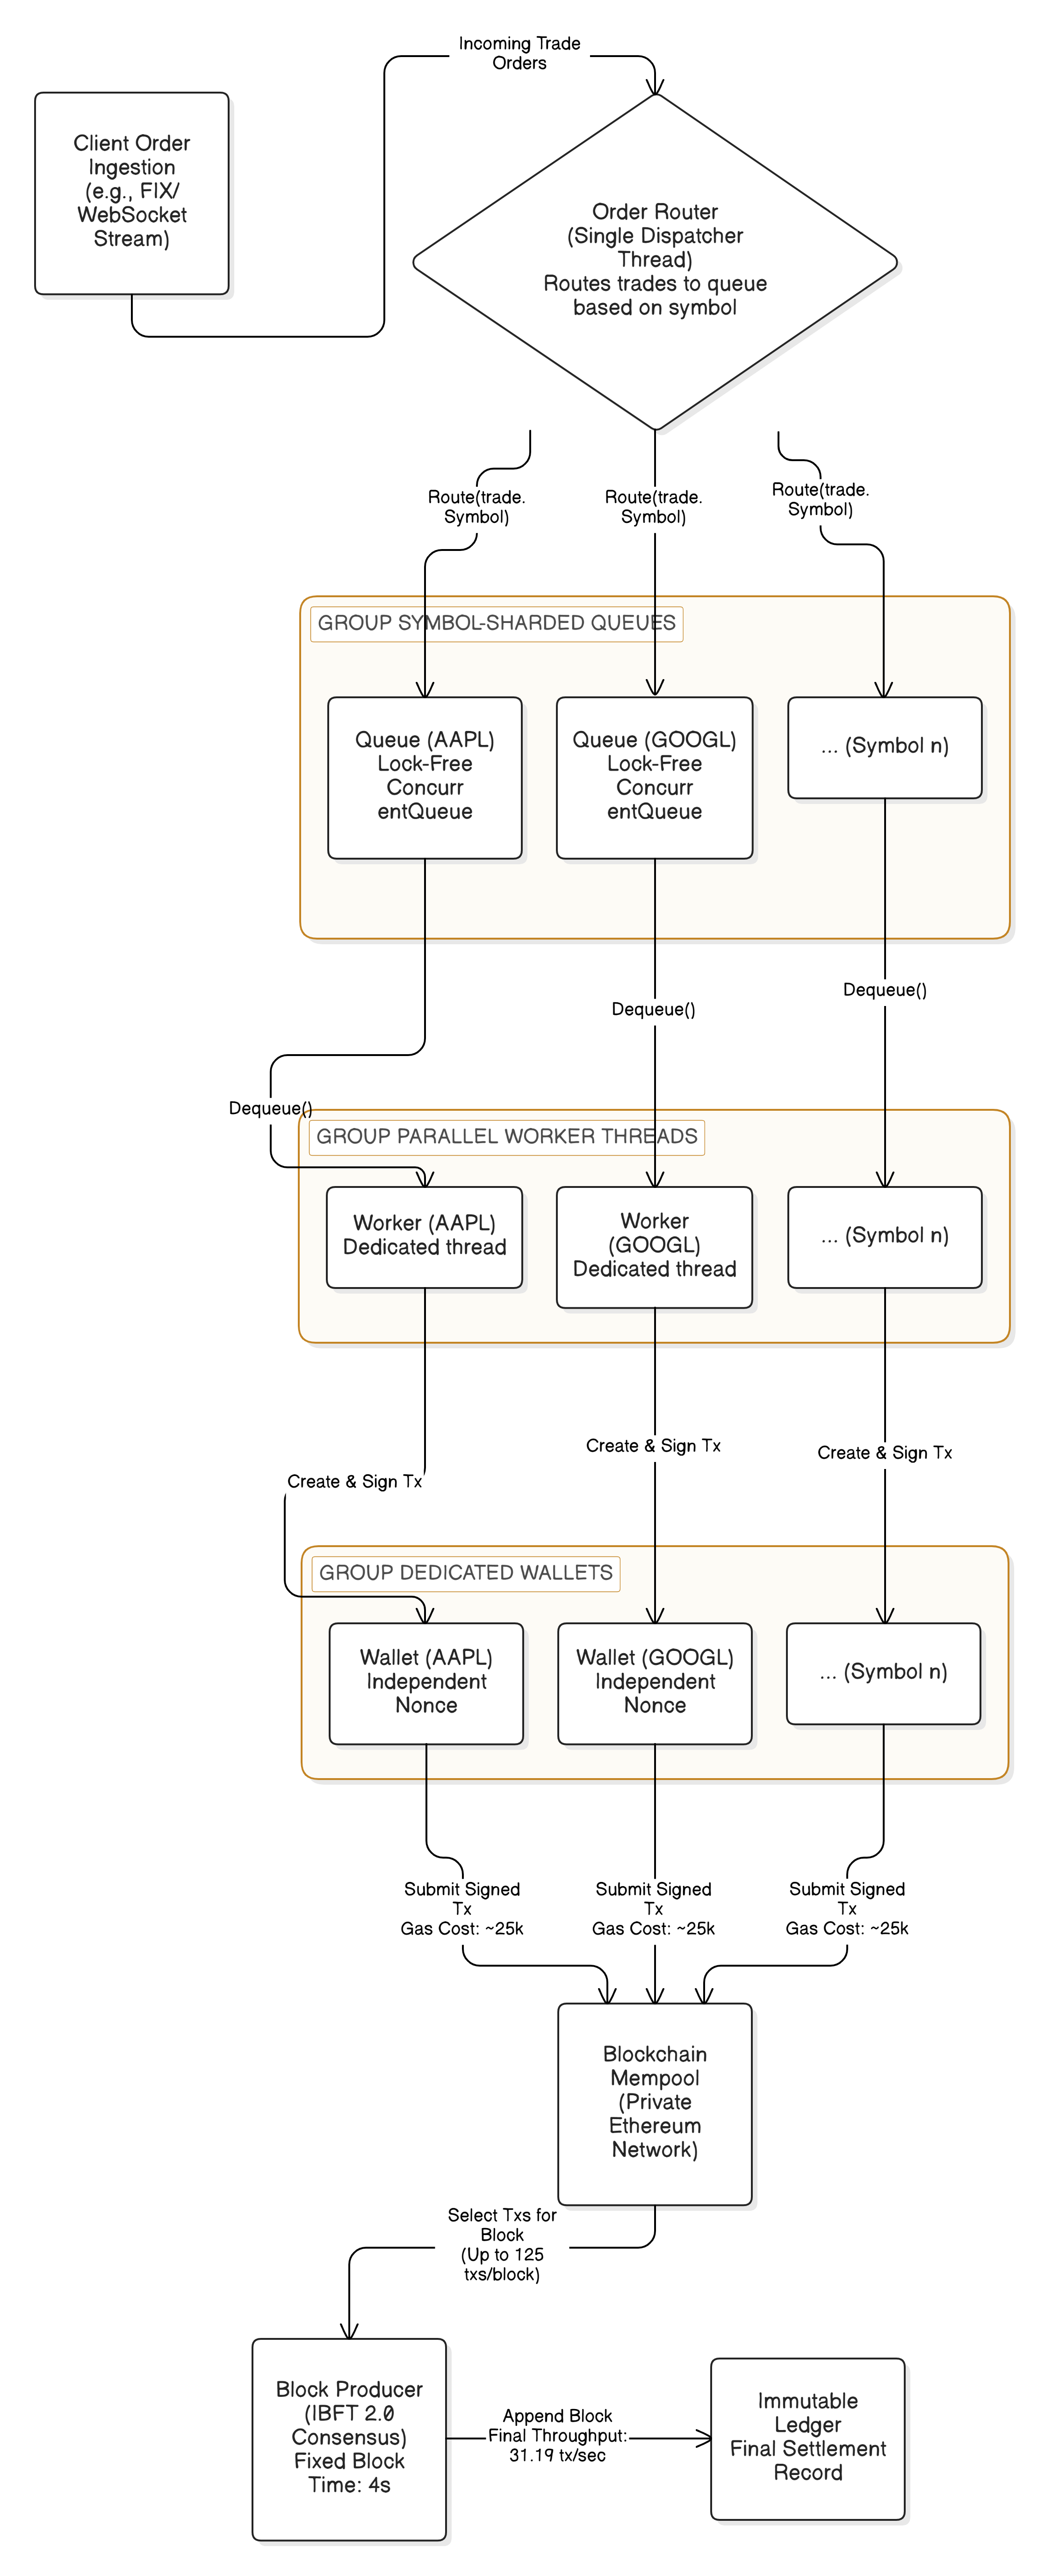
\includegraphics[height=0.65\textheight,keepaspectratio]{images/solution-architecture5.png}
\caption{Complete solution architecture integrating the Symbol-Sharded Lock-Free Model and the Asynchronous Multi-Wallet Strategy, achieving $\lambda_{max} = \lambda_{blockchain}$.}
\label{fig:solution-architecture}
\end{figure}
